\documentclass[12pt,a4paper]{article}

% Margins.
\setlength{\oddsidemargin}{0in}
\setlength{\evensidemargin}{0in}
\setlength{\headheight}{12pt}
\setlength{\headsep}{42pt}
\setlength{\topmargin}{-54pt}
\setlength{\textwidth}{6.5in}
\setlength{\textheight}{10in}

\usepackage{amsmath}
\usepackage{float}
\usepackage{graphicx}
\usepackage[hyphens]{url}
\usepackage{hyperref}	% Clickable links to figures, references and urls.
\usepackage{datetime}
\usepackage{longtable}
\usepackage{subfigure}

% Links direct to top of figures.
\usepackage[all]{hypcap}

% Drawing.
\usepackage{pgf}
\usepackage{tikz}

% Listings for formatting code.
\usepackage{listings}
\usepackage{textcomp}
% General options.+++
\lstset{breaklines=true, basicstyle=\small\ttfamily, tabsize=4, numbers=left, stepnumber=1, frame=single, showstringspaces=false, upquote=true}
% C++ specific high-lighting. Comments are 50/50 shades of green/black and strings coloured with 60/40 red/black mixture.
\lstset{language=[ISO]C++, commentstyle=\color{green!50!black}, keywordstyle=\color{blue}, stringstyle=\color{red!60!black}}

%opening
\title{\vspace{-3cm}Physics for Engineers\\Class 33\\Biot--Savart Law}
\author{Attique Dawood}
\date{April 10, 2014\\[0.2cm] Last Modified: \today, \currenttime}
\begin{document}
\maketitle
\section{Announcements}
\begin{itemize}
\item None.
\end{itemize}
\section{Biot--Savart Law}
Biot--Savart Law is the magnetostatics analogue of Coulomb's Law. The source of electrostatic field is a charge at rest. The source static magnetic field is a steady current (or DC current). When current flows in a wire a magnetic field is set up around the wire. The magnitude and direction of magnetic is given by the Biot--Savart Law
\begin{equation}
d\textbf{H}=\dfrac{Id\textbf{\textit{l}}\times(\textbf{r}-\textbf{r}')}{4\pi|\textbf{r}-\textbf{r}'|^{3}}.
\end{equation}
Or
\begin{equation}
d\textbf{B}=\dfrac{\mu_0Id\textbf{\textit{l}}\times(\textbf{r}-\textbf{r}')}{4\pi|\textbf{r}-\textbf{r}'|^{3}}.
\end{equation}
\section{Exercises}
\noindent\textbf{Question 1 \cite[Example 7.3, page 270]{Sadiku}:} A circular loop located on $x^2+y^2=9$, $z=0$ carries a direct current of 10 A along $\hat\phi$. Determine \textbf{H} at (0, 0, 4) and (0, 0, -4).\\[0.2cm]
\noindent\textbf{Question 2 \cite[PE 7.3, page 271]{Sadiku}:} A thin ring of radius 5 cm is placed on plane $z=1$ cm so that its centre is at (0, 0, 1 cm). If the ring carries 50 mA along $\hat\phi$, find \textbf{H} at
\begin{itemize}
\item[a.] (0 ,0, -l cm)
\item[b.] (0 ,0, 10 cm)
\end{itemize}
%\begin{itemize}
%\item[a.] Electric field of a point charge.
%\item[b.] Electric field of an infinite line charge placed along $z$--axis.
%\end{itemize}
%%\begin{figure}[H]
%\centering
%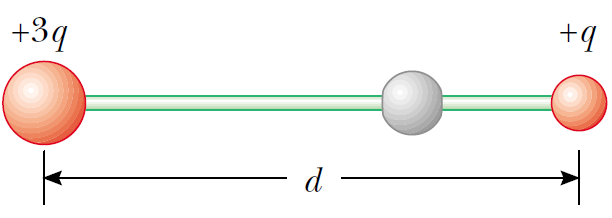
\includegraphics[scale=0.45]{FigureP23-10.png}
%\caption{Equilibrium of charge.}
%\label{Equilibrium}
%\end{figure}
%\nocite{*}
\bibliographystyle{plain}
\bibliography{PhysicsRef}
\end{document}
